\chapter{RESULTS}
\pagestyle{fancy}

In this chapter, we present the results from our proposed method. The following parts of this chapter is organized as follows: In section 4.1, we briefly introduce our experiment settings, and present the test results. Section 4.2 gives a demonstration on how we can apply our model in identifying airport delay connections based on the data from single operation day. Finally, we extend our model to investigate daily connection in section 4.3 and present the estimation.

\section{Experiments}

We assess the performance of our model in terms of both graph clustering and connection identification. 

\noindent\textbf{Baselines.} To demonstrate the power of integrating graph learning in the framework, we compare our clustering results with ones obtained using multiple predefined adjacency matrices $A_1, A_2, A_3$. Denote the great circle distance between airport $i$ and $j$ by $D_{ij}$, and the number of inter-airport flights by $N_{ij}$, we construct these adjacency matrices as follows:
\begin{equation}
    \left[A_1\right]_{ij}=\frac{1}{2}(D_{ij}+N_{ij})
\end{equation}
\begin{equation}
    \left[A_2\right]_{ij}=\frac{1}{3}(D_{ij}+2N_{ij})
\end{equation}
\begin{equation}
    \left[A_3\right]_{ij}=\frac{1}{3}(2D_{ij}+N_{ij})
\end{equation}

\noindent\textbf{Metrics.} We measure the performance of the graph clustering model using graph-level metrics: average cluster conductance \citep{yang2015defining} and graph modularity \citep{newman2006modularity}. The conductance of a cluster is defined as the fraction of total inter-cluster edge weights. We use the average level of all clusters as our performance measure and expect a low overall conductance.
\begin{equation}
    \mathcal{C}=\frac{1}{|C|}\frac{\sum_C\sum_{i\in C,j\notin C}w_{ij}}{\sum_i\sum_j w_{ij}}
\end{equation}

The graph modularity measures the sparse and dense structure of clusters compare to a random graph. A higher modularity refers to a better clustering structure.
\begin{equation}
    \mathcal{Q}=\frac{1}{C}\sum_{A_i,i\in C}\frac{1}{2m}\left(A_i-\frac{d_id_i^\intercal}{2m}\right)
\end{equation}

We fix the architecture for all clustering networks to have one hidden layer with 64 neurons in it and set the number of target clusters to 16. We use ADAM optimizer with a learning rate of 0.001 and train our model for 1000 epochs. The results are in \hyperref[tab:4-1]{Table 4.1}.

\begin{table}[thbp]
    \label{tab:4-1}
    \caption{Results of Experiments}
    \centering
    \begin{tabular}{@{}ccccccc@{}}
    \toprule
    \textbf{Features} &
      \multicolumn{2}{c}{\textbf{Dep. Delay}} &
      \multicolumn{2}{c}{\textbf{Arr. Delay}} &
      \multicolumn{2}{c}{\textbf{Dep. \& Arr. Delay}} \\ \midrule
    \textbf{Method} & $\mathcal{C}\downarrow$     & $\mathcal{Q}\uparrow$      & $\mathcal{C}\downarrow$ & $\mathcal{Q}\uparrow$      & $\mathcal{C}\downarrow$ & $\mathcal{Q}\uparrow$      \\
    GCN + $A_1$        & 0.7962          & -0.0173         & 0.6977      & -0.0133         & 0.5237      & -0.0184         \\
    GCN + $A_2$        & 0.8092          & -0.0220         & 0.7193      & -0.0216         & 0.5545      & -0.0227         \\
    GCN + $A_3$        & 0.7859          & -0.0140         & 0.6756      & -0.0077         & 0.5143      & -0.0149         \\
    \textbf{ADMoN}  & \textbf{0.2882} & \textbf{0.4110} & 0.6831      & \textbf{0.1521} & 0.5711      & \textbf{0.2554} \\ \bottomrule
    \end{tabular}
\end{table}

Judging by only the modularity, our model has a significantly better performance over those with predefined adjacency matrices, which indicates that graph learning can indeed help extrapolate the latent sparse connections based on delay features. We believe predefined adjacency matrices failed because they are not sparse enough to support graph clustering. Besides, results on dataset with only departure delay are significantly better than those with arrival delay. We believe this is due to the fact that arrival delay are to some extent affected by en-route conditions (e.g., winds, rains, etc.) which leads to variance in delay features.

\section{Airport Connection Identification}
In this section, we use a daily-level example to demonstrate how we can apply our model to identify airport delay connections based on the data from single operation day. 

\hyperref[tab:4-2]{Table 4.2} shows the airport cluster of Jul.8, 2019. To better illustrate, we draw a map to show the location of airports in \hyperref[fig:4-1]{Figure 4.1}. The color of nodes represent the cluster. The strength of connections between airports are shown in \hyperref[fig:4-2]{Figure 4.2}. We can see that clusters of airports are not purely identified by their locations. We suppose that similar airport daily delay patterns results from two aspects. First, multiple airports within a geographical region will simultaneously experience flight delays, when convective weather cover this area. Second, for other airports that are not directly affected by the weather, they will experience time lagged propagated delay by direct flights. So, results of \hyperref[fig:4-1]{Figure 4.1} indicate propagated delay by direct flights also matter in airport delay patterns. 

\begin{table}[thbp]
    \label{tab:4-2}
    \caption{Airport Clusters of Jul 8, 2019}
    \centering
    \begin{tabular}{@{}cl@{}}
    \toprule
    \textbf{Cluster No.} & \multicolumn{1}{c}{\textbf{Airports}} \\ \midrule
    \textbf{1}           & ATL, BOS, BWI, CLT, EWR, IAH, LAS     \\
    \textbf{2}           & DCA, DFW, DTW, FLL, JFK               \\
    \textbf{3} & \begin{tabular}[c]{@{}l@{}}IAD, LAX, LGA, MCO, MDW, MEM, MIA, MSP,\\ ORD, PHL, PHX, SAN, SEA, SFO, SLC, TPA\end{tabular} \\
    \textbf{4}           & DEN                                   \\ \bottomrule
    \end{tabular}
\end{table}

\begin{figure}[thbp]
    \label{fig:4-1}
    \centering
    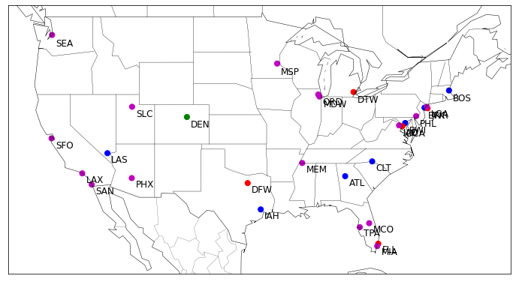
\includegraphics[width=\textwidth]{img/map of cluster.png}
    \caption{Airport clusters and locations on map (Jul.8)}
\end{figure}

\begin{figure}[t!]
    \label{fig:4-2}
    \centering
    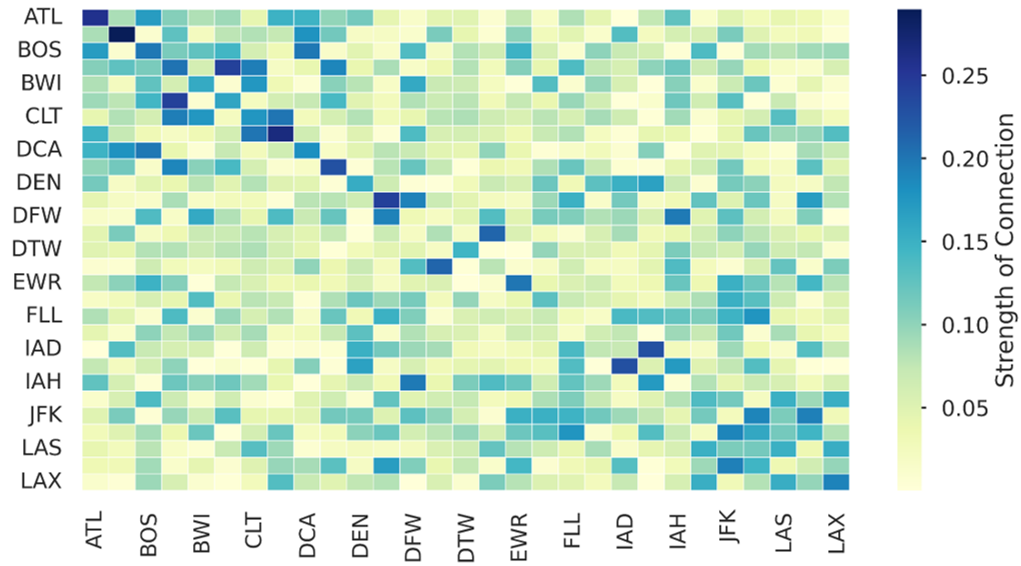
\includegraphics[width=\textwidth]{img/adjacency.png}
    \caption{Strength of Connections Between Airports (Jul.8)}
\end{figure}

We then further examine see why these airports are identified in one cluster, by looking at the departure delay excess accumulation.  \hyperref[fig:4-3]{Figure 4.3} shows the time series of departure delay excess accumulation of each airport in different clusters. In cluster 1, the airport excess accumulation is high during 0:00-04:00, and 19:00-23:59. In cluster 2, there is a relatively small accumulation during 0:00-1:00, and a high accumulation starts from the noon. In addition, in cluster 1 and 2, we can find the time series of accumulation these two clusters show some latent ‘time-lagged’ pattern, which indicates that the airports in these 2 clusters have similar patterns because of propagated delay. In each cluster, there is one airport has extreme large excess accumulation. The time series of other airports follow the pattern of this airport. We suspect that the airport with extreme large excess accumulation experienced server disruptions, and other airports are affected by the propagated flights delay. In cluster 3, the overall magnitude of excess accumulation is smaller, but the duration is longer than the other clusters. It shows that there are continual congestion at these airports during the daytime. By looking at the map, these airports are geographically close, such as TPA, MIA and MCO in the southeast coast. The continual accumulation during daytime suggests that these airports may have demand and capacity imbalance problem. Cluster 4 may be the outlier.

\begin{figure}[thbp]
    \label{fig:4-3}
    \centering
    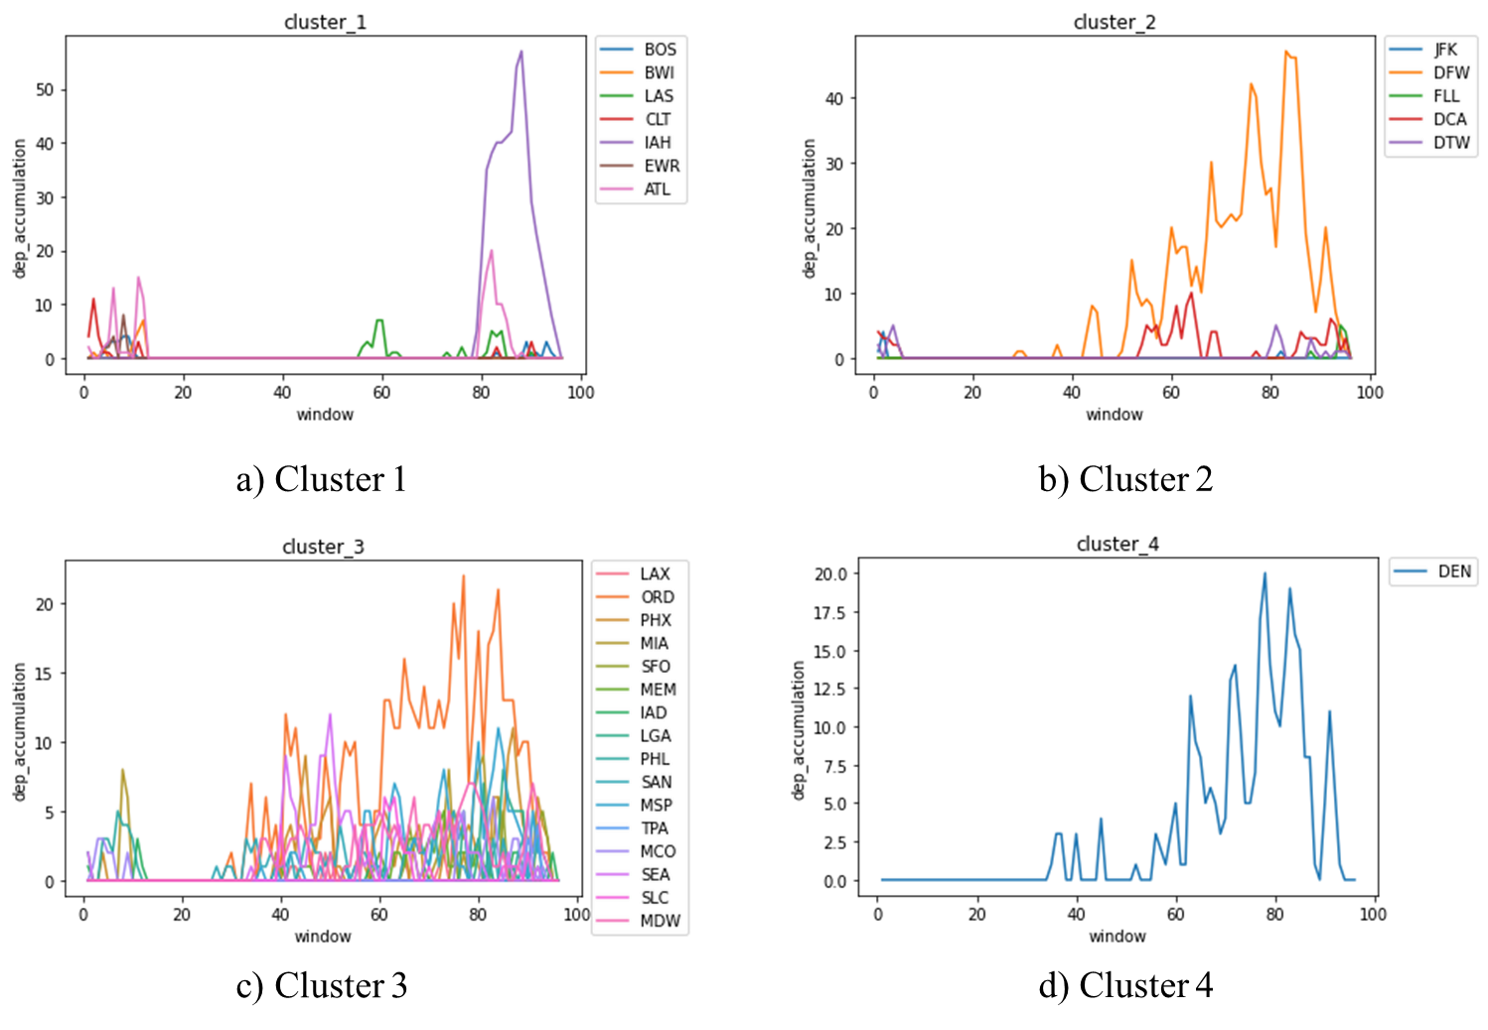
\includegraphics[width=\textwidth]{img/4 clusters.png}
    \caption{Time Series of Departure Delay Excess Accumulation (Jul.8)}
\end{figure}

We also look at the clustering results of Aug.5, 2019. The airport clusters and strength of connections are shown in \hyperref[tab:4-3]{Table 4.3} and \hyperref[fig:4-4]{Figure 4.4} respectively. Compared with \hyperref[tab:4-2]{Table 4.2} and \hyperref[fig:4-2]{Figure 4.2}, we find that some airports are in the cluster in two different days, e.g. SFO, SLC, PHX, SAN,and SEA; ATL and CLT, TPA, MCO and MIA. It motivates us to investigate the daily connextions.

\begin{table}[thbp]
    \label{tab:4-3}
    \caption{Airport Clusters of Aug 5, 2019}
    \centering
    \begin{tabular}{@{}cl@{}}
    \toprule
    \textbf{Cluster No.} & \multicolumn{1}{c}{\textbf{Airports}} \\ \midrule
    \textbf{1}           & IAD,MCO,MDW,MEM,MIA,MSP,ORD,PHL,PHX,SAN,SEA,SFO,SLC,TPA     \\
    \textbf{2}           & LAX, LGA              \\
    \textbf{3} & \begin{tabular}[c]{@{}l@{}}EWR, IAH, JFK, LAS\end{tabular} \\
    \textbf{4}           & ATL, BOS, BWI, CLT, DCA, DEN, DFW, DTW, FLL                                   \\ \bottomrule
    \end{tabular}
\end{table}

\begin{figure}[t!]
    \label{fig:4-4}
    \centering
    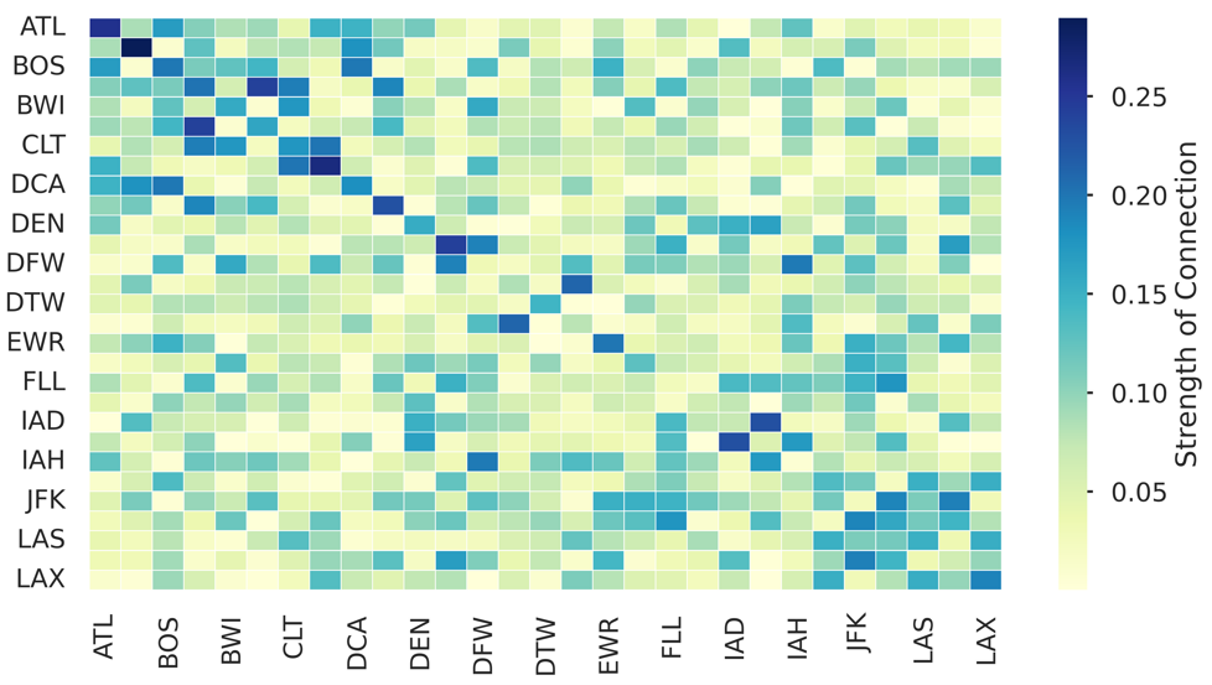
\includegraphics[width=\textwidth]{img/strength 0805.png}
    \caption{ Strength of Connections Between Airports  (Aug.5)}
\end{figure}

\section{Daily Connection Identification}

As mentioned in section 3.3.3, by using the eigenvalues of identified adjacency matrices as our new input features, our model can identify connections among operation days. 

\hyperref[fig:4-5]{Figure 4.5} shows the identification result. Overall, most of the operational days share similarities with each other, which is demonstrated by the background noises. Near the diagonal, we can see clusters at early July, mid-August, and early September. Strong connections can be see in these periods for days in the same week. But compared to the background noise, the strengths are insignificant.

\begin{figure}[thbp]
    \centering
    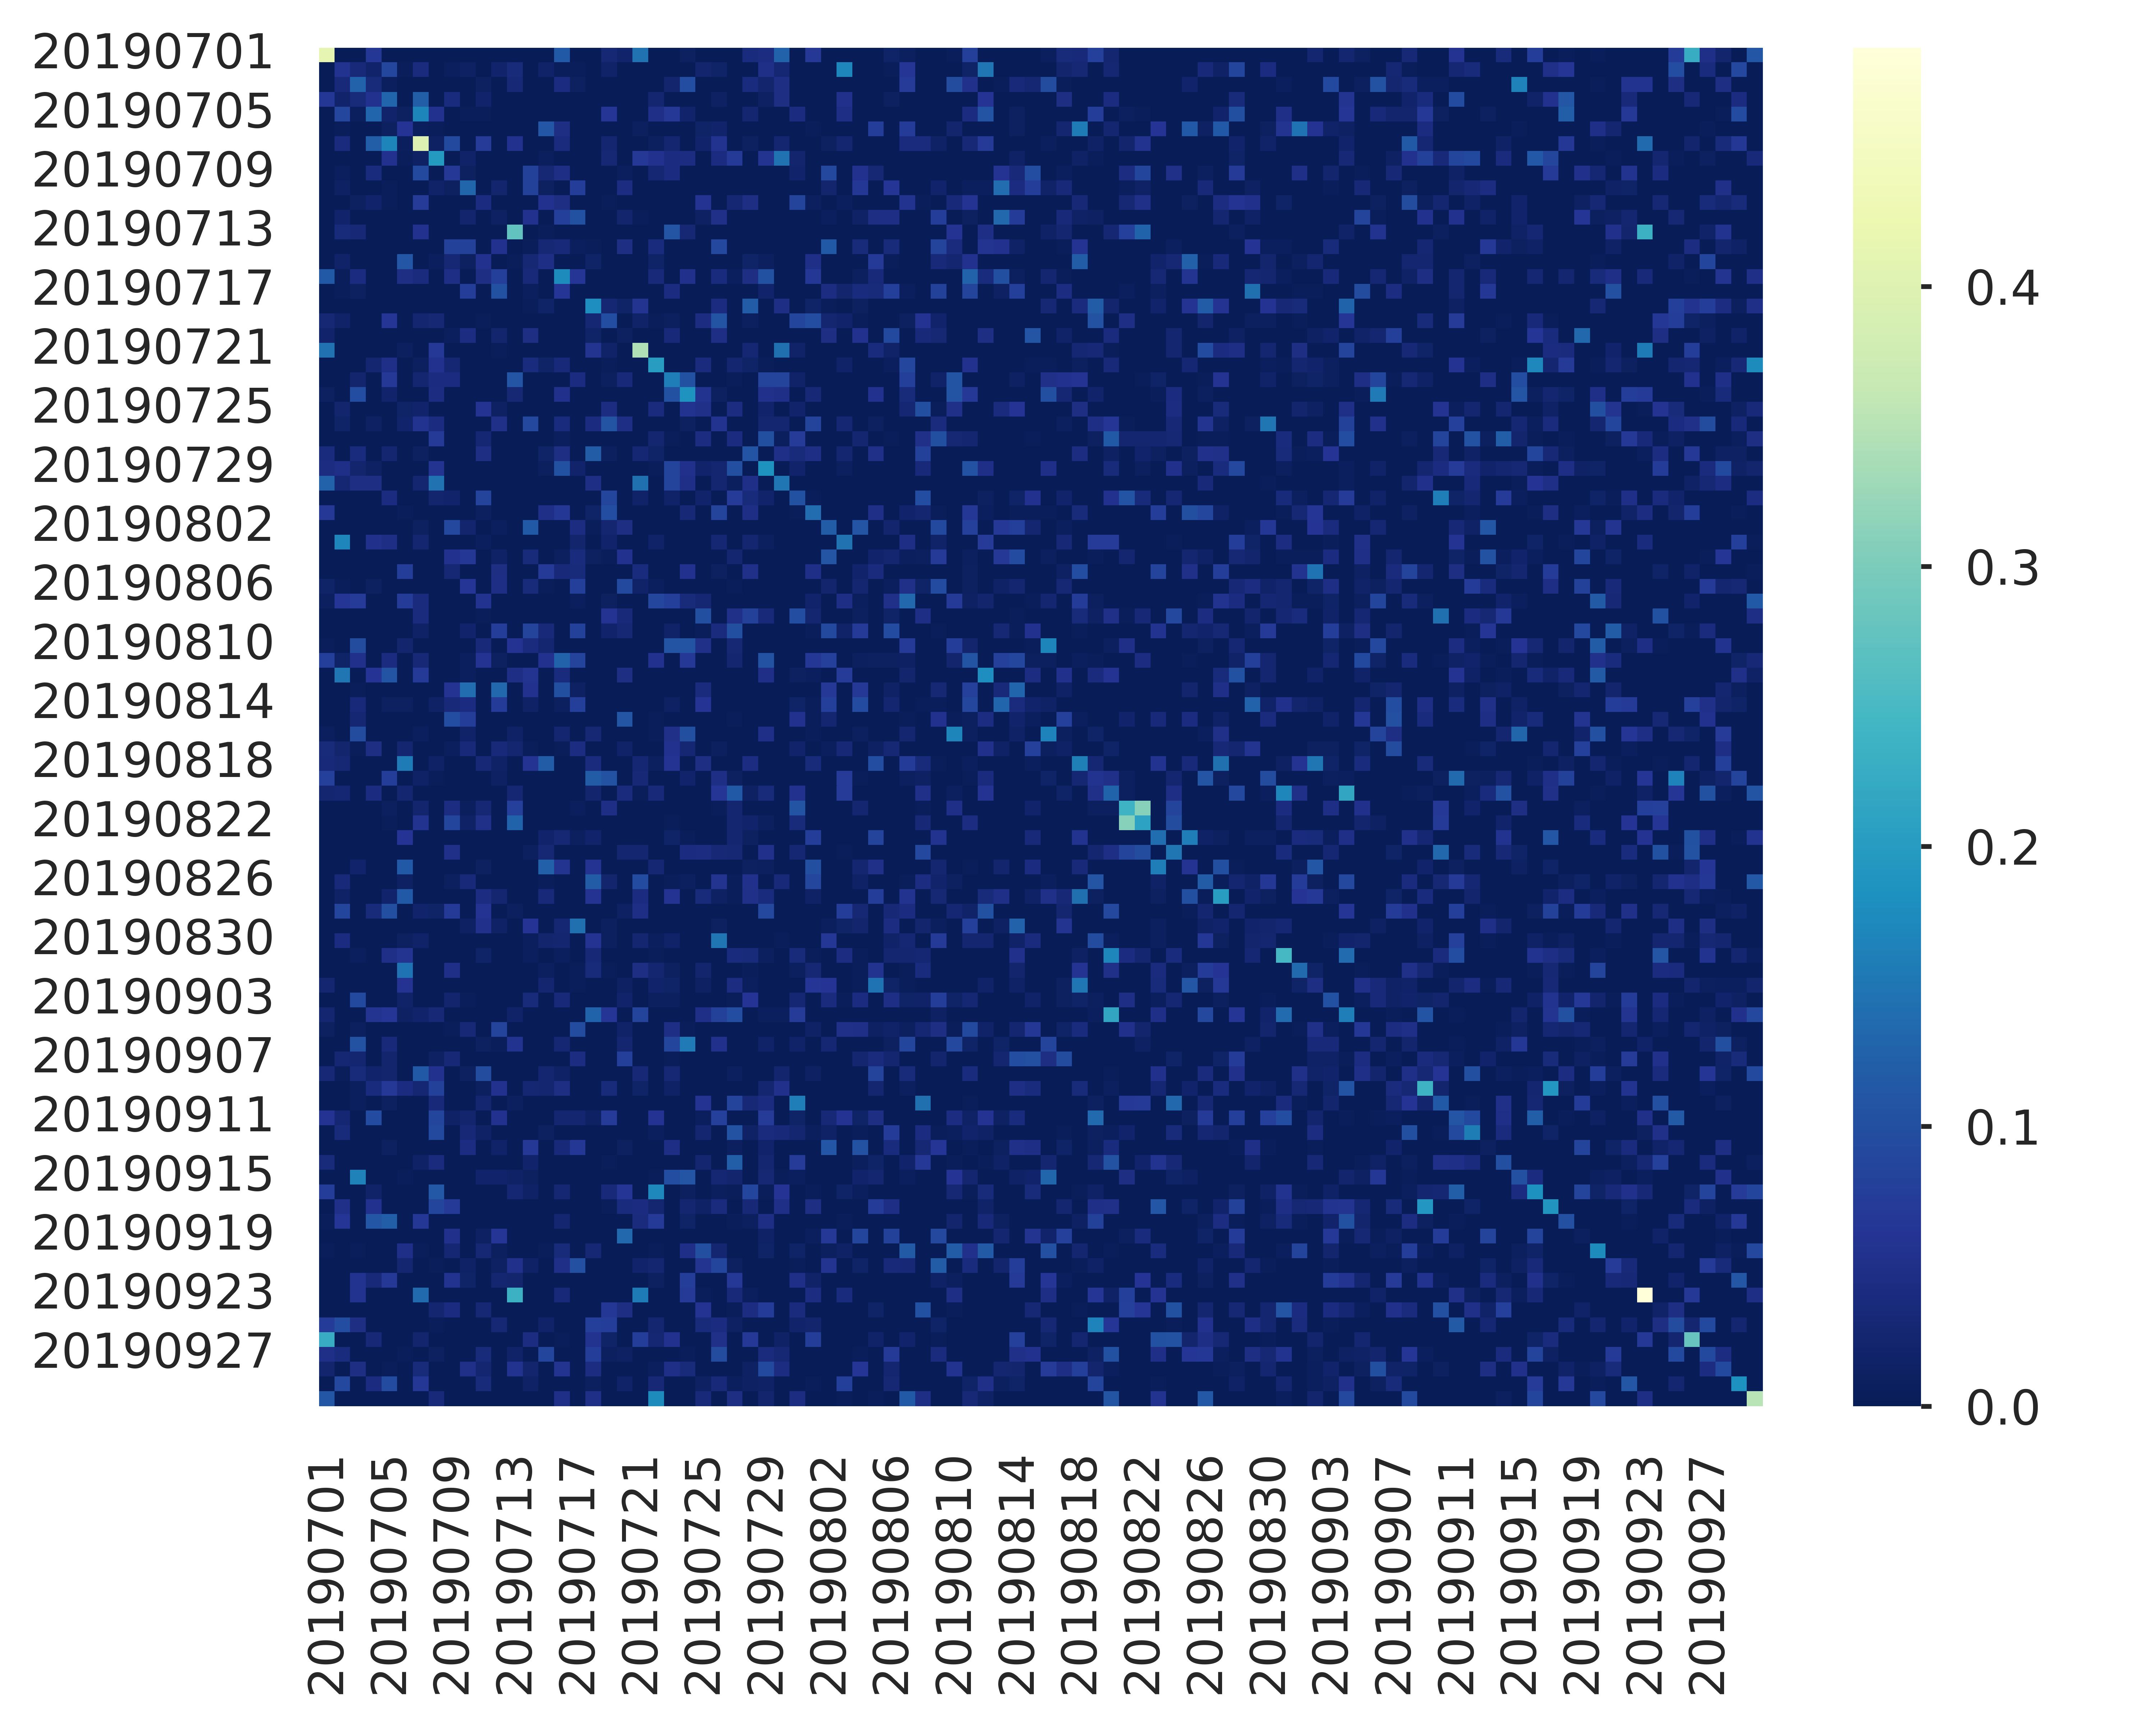
\includegraphics[width=\textwidth]{img/daily_corr.png}
    \caption{Strength of Connections Between Operation Days}
    \label{fig:4-5}
\end{figure}

% \begin{tcolorbox}[breakable,title={An example colorbox},
% colback=founderblue!5!white,
% colframe=founderblue!75!black,
% fonttitle=\headingfont\bfseries\large]
% Your text goes here. The colors are based on Berkeley's Founder Blue.
% \tcbsubtitle[before skip=\baselineskip]%
% {You can also have subboxes}
% Don't like the colors? You can change them here (replace founderblue with the color you like), or you can change them globally in the colors section of report.tex
% \tcbsubtitle[before skip=\baselineskip]%
% {Multiple rows}
% If you like it.
% \end{tcolorbox}